\documentclass[10pt]{beamer}

% ------------------------------------------------------------------------
% Carga de tu preámbulo personalizado (preamble.tex).
% Asegúrate de tenerlo en la misma carpeta para que \input funcione.
% ------------------------------------------------------------------------
\usetheme[progressbar=frametitle]{metropolis}
\usepackage{appendixnumberbeamer}
\usepackage{fancyvrb}
\usepackage{booktabs}
\usepackage[scale=2]{ccicons}
\usepackage{pgfplots}
\usepgfplotslibrary{dateplot}
\usepackage{type1cm}
\usepackage{lettrine}
\usepackage{ragged2e}
\usepackage{xspace}
\newcommand{\themename}{\textbf{\textsc{metropolis}}\xspace}
\usepackage{graphicx} % Allows including images
\usepackage{booktabs} % Allows the use of \toprule, \midrule and \bottomrule in tables
\usepackage[utf8]{inputenc} %solucion del problema de los acentos.
\usepackage{xcolor}
\definecolor{LightGray}{gray}{0.9}

\usepackage{minted}
\usemintedstyle{tango}
\newcommand{\mypyfile}[1]{\inputminted[linenos=true, fontsize=\footnotesize, frame=lines, framesep=5\fboxrule,framerule=1pt]{python}{#1}}

\setminted[python]{breaklines,frame=lines,framesep=2mm,baselinestretch=1.2,bgcolor=LightGray,linenos, fontsize=\footnotesize} % obeytabs=true, tabsize=2, showtabs=true}

%%%%%%%%%%%%%%%%%%%%%%%%%%%%%%%%%%%%%%%%%%%%%%%%%%%%%%%%%%%%%%%%%%%%%%%%%%%%%%%%%%%%%%
\setbeamercolor{progress bar}{fg=blue!50!black,bg=white!50!black}
\setbeamercolor{title separator}{fg=red!50!black,bg=white!50!black}
\setbeamercolor{frametitle}{fg=white!80!black,bg=red!50!black}
\title[PCFI161]{Programaci\'on para F\'isica y Astronom\'ia}
\subtitle{Departamento de Física.}

\newcommand{\myfront}{
\author[PCFI161]{Corodinadora: C Loyola \\ Profesoras/es C Loyola / C Femenías / Y Navarrete / C Ruiz}
\institute[UNAB]{Universidad Andrés Bello}
\date{Primer Semestre 2025}
}

\titlegraphic{%
  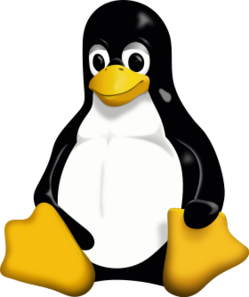
\includegraphics[width=.08\textwidth]{logo-tux.png}\hfill
  
\includegraphics[width=.3\textwidth]{logo-unab.png}\hfill
  
\includegraphics[width=.08\textwidth]{logo-python.png}
}

\makeatletter
\setbeamertemplate{title page}{
  \begin{minipage}[b][\paperheight]{\textwidth}
    \vfill%
    \ifx\inserttitle\@empty\else\usebeamertemplate*{title}\fi
    \ifx\insertsubtitle\@empty\else\usebeamertemplate*{subtitle}\fi
    \usebeamertemplate*{title separator}
    \ifx\beamer@shortauthor\@empty\else\usebeamertemplate*{author}\fi
    \ifx\insertdate\@empty\else\usebeamertemplate*{date}\fi
    \ifx\insertinstitute\@empty\else\usebeamertemplate*{institute}\fi
    \vfill
    \ifx\inserttitlegraphic\@empty\else\inserttitlegraphic\fi
    \vspace*{1cm}
  \end{minipage}
}
\makeatother


\makeatletter
\setlength{\metropolis@titleseparator@linewidth}{2pt}
\setlength{\metropolis@progressonsectionpage@linewidth}{2pt}
\setlength{\metropolis@progressinheadfoot@linewidth}{2pt}
\makeatother


\begin{document}

% ------------------------------------------------------------------------
% Portada de la Presentación
% ------------------------------------------------------------------------
\myfront{}

% ------------------------------------------------------------------------
% Slide 1: Título de la Sesión
% ------------------------------------------------------------------------
\begin{frame}
  \titlepage
  % Por ejemplo:
  % \title{Semana 11 - Sesión 2 (Sesión 22): Proyectos Colaborativos y Retroalimentación}
\end{frame}

% ------------------------------------------------------------------------
% Slide 2: Índice / Tabla de Contenidos
% ------------------------------------------------------------------------
\begin{frame}
  \frametitle{Resumen - Semana 11, Sesión 2 (Sesión 22)}
  \tableofcontents
\end{frame}

% ------------------------------------------------------------------------
% Configuración de bloques
% ------------------------------------------------------------------------
\metroset{block=fill}

% ----------------------------------------------------------------------------------------
% SECCIÓN 1: Introducción y Conexión con la Sesión Anterior
% ----------------------------------------------------------------------------------------
\section{Introducción y Contexto}

% ------------------------------------------------------------------------
% Slide 3: Conexión con Semana 11, Sesión 1
% ------------------------------------------------------------------------
\begin{frame}{Contexto Tras la Solemne II (Continuación)}
  \begin{itemize}
    \item \textbf{Semana 11, Sesión 1 (Sesión 21)}:
      \begin{itemize}
        \item Retroalimentación general de la Solemne II.
        \item Profundización en \textbf{POO avanzada}: polimorfismo, composición.
        \item Propuesta de ejemplos físicos (Body, Star, SolarSystem).
      \end{itemize}
    \item \textbf{Semana 11, Sesión 2 (Sesión 22)}:
      \begin{itemize}
        \item Podríamos comenzar a plantear \textbf{proyectos colaborativos} o la fase final del curso, dependiendo del Syllabus.
        \item Seguir revisando retroalimentación \textbf{individual} y plan de recuperación si alguien necesita.
      \end{itemize}
    \item \textbf{Objetivo de hoy}: Organizar ideas para trabajos/proyectos finales, o ejercicios de refuerzo según la ruta del Syllabus.
  \end{itemize}
\end{frame}

% ------------------------------------------------------------------------
% Slide 4: Objetivos de la Sesión 22
% ------------------------------------------------------------------------
\begin{frame}{Objetivos de la Sesión 22}
  \begin{itemize}
    \item \textbf{Compartir} retroalimentación más detallada de la Solemne II a nivel individual (cuando corresponda).
    \item \textbf{Proponer} líneas de trabajo para un \textbf{proyecto integrador} (o mini-proyecto), combinando POO y análisis de datos.
    \item \textbf{Fomentar} la discusión y asignación de \textbf{equipos} o \textbf{temáticas}, si es un proyecto grupal.
    \item \textbf{Refrescar} cualquier duda sobre polimorfismo, composición u otros temas recientes.
  \end{itemize}
\end{frame}

% ----------------------------------------------------------------------------------------
% SECCIÓN 2: Retroalimentación Individual de la Solemne II
% ----------------------------------------------------------------------------------------
\section{Retroalimentación Individual}

% ------------------------------------------------------------------------
% Slide 5: Acceso a Retroalimentación en CANVAS
% ------------------------------------------------------------------------
\begin{frame}{Acceso a Retroalimentación}
  \begin{itemize}
    \item \textbf{Notas y comentarios} ya publicadas en CANVAS.
    \item Revisen su \textbf{archivo corregido} (o PDF de correcciones) para ver comentarios específicos.
    \item \textbf{Pregunten} si hay dudas sobre la calificación o la forma de mejorar.
  \end{itemize}
\end{frame}

% ------------------------------------------------------------------------
% Slide 6: Estadísticas Adicionales (si aplica)
% ------------------------------------------------------------------------
\begin{frame}{Estadísticas Adicionales}
  \begin{itemize}
    \item Medias y desv. estándar de notas, si corresponde.
    \item Observaciones sobre \textbf{tiempo} y \textbf{estrategia} de resolución.
    \item Tipos de errores frecuentes:
      \begin{itemize}
        \item Falta de \textbf{super()} en herencia.
        \item Errores de \textbf{reshape} en NumPy o confusión en subplots.
        \item Falta de validación en \textbf{pandas} (CSV mal formateados).
      \end{itemize}
  \end{itemize}
\end{frame}

% ----------------------------------------------------------------------------------------
% SECCIÓN 3: Proyectos o Ejercicios Finales
% ----------------------------------------------------------------------------------------
\section{Proyectos Finales}

% ------------------------------------------------------------------------
% Slide 7: Propuesta de Proyecto Integrador
% ------------------------------------------------------------------------
\begin{frame}{Propuesta de Proyecto Integrador (Ejemplo)}
  \begin{block}{Idea General}
    \begin{itemize}
      \item \textbf{Objetivo}: desarrollar un mini-proyecto donde se combinen:
        \begin{itemize}
          \item \textbf{POO} para modelar entidades (partículas, cuerpos astronómicos, datos experimentales).
          \item \textbf{NumPy} para cálculos numéricos (simulaciones, estadísticas).
          \item \textbf{Matplotlib} para visualización 2D/3D.
          \item (Opcional) \textbf{pandas} para manejo de datos más robusto (CSV, merges, etc.).
        \end{itemize}
      \item \textbf{Equipo}: 2-3 personas, entregando un \textbf{repositorio} o un \textbf{notebook} en Colab con explicación.
      \item \textbf{Extensión}: ~1-2 semanas de desarrollo, con check-ins intermedios.
    \end{itemize}
  \end{block}
\end{frame}

% ------------------------------------------------------------------------
% Slide 8: Ejemplos de Temáticas
% ------------------------------------------------------------------------
\begin{frame}{Temáticas Suggeridas}
  \begin{itemize}
    \item \textbf{Simulación de órbitas} en un sistema planetario simple (\texttt{Body}, \texttt{SolarSystem}).
    \item \textbf{Modelo de cargas} (Particle, ChargedParticle) e interacción electrostática.
    \item \textbf{Análisis de datos experimentales} con una clase \texttt{Measurement} y comparaciones estadísticas en \textbf{pandas}.
    \item \textbf{Animaciones} con Matplotlib (\texttt{FuncAnimation}) de un movimiento 2D/3D.
    \item Cualquier otra idea relevante al campo de Física/Astronomía/Ingeniería.
  \end{itemize}
\end{frame}

% ------------------------------------------------------------------------
% Slide 9: Organización y Entregables
% ------------------------------------------------------------------------
\begin{frame}{Organización del Proyecto (si aplica)}
  \begin{itemize}
    \item \textbf{Formación de grupos}: 2-3 integrantes.
    \item \textbf{Plan de trabajo}:
      \begin{itemize}
        \item Propuesta inicial (alcances, clases a definir, datos a usar).
        \item Avance parcial (estructuras POO, prototipos de gráficas).
        \item Entrega final (documentación en un \textbf{README} o en celdas de \textbf{Markdown}).
      \end{itemize}
    \item \textbf{Evaluación}:
      \begin{itemize}
        \item Organización y claridad del código (POO, funciones auxiliares).
        \item Uso correcto de NumPy/Matplotlib/pandas según corresponda.
        \item Resultados coherentes, gráficas interpretables.
        \item Documentación y conclusiones (Markdown o PDF anexo).
      \end{itemize}
  \end{itemize}
\end{frame}

% ----------------------------------------------------------------------------------------
% SECCIÓN 4: Reforzando Temas Pendientes
% ----------------------------------------------------------------------------------------
\section{Refuerzo de Temas Pendientes}

% ------------------------------------------------------------------------
% Slide 10: Recopilación de Dudas
% ------------------------------------------------------------------------
\begin{frame}{Recopilación de Dudas Pendientes}
  \begin{itemize}
    \item \textbf{POO avanzada}: polimorfismo, composición, encapsulación relativa en Python.
    \item \textbf{NumPy}: broadcast, random, performance tips.
    \item \textbf{Matplotlib}: subplots 3D, animación (FuncAnimation), personalización avanzada (fonts, styles).
    \item \textbf{pandas}: merges, groupby, time-series (si aplica).
  \end{itemize}
  \textbf{Comparte tus inquietudes en voz alta o en foros.}
\end{frame}

% ------------------------------------------------------------------------
% Slide 11: Minicharla: Animaciones en Matplotlib (si hay tiempo)
% ------------------------------------------------------------------------
\begin{frame}[fragile]{Minicharla: Animaciones (Opcional)}
\begin{itemize}
  \item Usar \(\texttt{matplotlib.animation.FuncAnimation}\).
  \item Estructura típica:
\begin{minted}{python}
import matplotlib.animation as animation

fig, ax = plt.subplots()
line, = ax.plot([], [], 'o-')

def init():
    ax.set_xlim(0, 10)
    ax.set_ylim(-1, 1)
    return line,

def update(frame):
    xdata.append(frame)
    ydata.append(np.sin(frame))
    line.set_data(xdata, ydata)
    return line,

ani = animation.FuncAnimation(fig, update,
                              frames=np.linspace(0,10,50),
                              init_func=init, blit=True)
plt.show()
\end{minted}
  \item \textbf{Aplicación}: movimiento de partículas, órbitas, propagación de ondas, etc.
\end{itemize}
\end{frame}

% ----------------------------------------------------------------------------------------
% SECCIÓN 5: Conclusiones y Próximos Pasos
% ----------------------------------------------------------------------------------------
\section{Conclusiones y Próximos Pasos}

% ------------------------------------------------------------------------
% Slide 12: Discusión de Próximos Proyectos
% ------------------------------------------------------------------------
\begin{frame}{Discusión Abierta}
  \begin{itemize}
    \item ¿Qué proyecto integrador les interesa más?
    \item ¿Necesitan datos reales (CSV) o preferirían algo 100\% simulado (NumPy random)?
    \item ¿Prefieren foco en \textbf{POO} o en \textbf{análisis/visualización}?
    \item \textbf{Objetivo} de la discusión: definir \textbf{lineamientos} finales del proyecto (o mini-tarea).
  \end{itemize}
\end{frame}

% ------------------------------------------------------------------------
% Slide 13: Conclusiones de la Sesión 22
% ------------------------------------------------------------------------
\begin{frame}{Conclusiones de la Sesión 22}
  \begin{itemize}
    \item Continuamos con la retroalimentación de la Solemne II, ahora a nivel \textbf{individual} y con consejos puntuales.
    \item Iniciamos la \textbf{planificación} de proyectos finales o colaborativos, unificando POO y análisis de datos.
    \item Reforzamos la disponibilidad de \textbf{espacios de dudas} para temas pendientes (polimorfismo, animaciones, etc.).
  \end{itemize}
\end{frame}

% ------------------------------------------------------------------------
% Slide 14: Próxima Sesión (Semana 12)
% ------------------------------------------------------------------------
\begin{frame}{Próximos Temas}
  \begin{itemize}
    \item \textbf{Semana 12}: Puesta en marcha de proyectos (si corresponde) o siguientes unidades del Syllabus.
    \item Revisar la \textbf{fechas} de entrega intermedia (si se establece).
    \item Seguir explorando \textbf{animaciones}, \textbf{estadística avanzada}, o \textbf{paralelización} (según plan).
  \end{itemize}
\end{frame}

% ------------------------------------------------------------------------
% Slide 15: Recursos Adicionales
% ------------------------------------------------------------------------
\begin{frame}{Recursos Adicionales}
  \begin{itemize}
    \item \href{https://realpython.com/courses/}{\textbf{Real Python}} - Sección de proyectos y guías prácticas.
    \item \href{https://matplotlib.org/stable/api/animation_api.html}{\textbf{Matplotlib Animation API}} - documentación oficial.
    \item \href{https://numpy.org/doc/stable/reference/routines.random.html}{\textbf{NumPy random}} - generadores pseudoaleatorios avanzados.
    \item \textbf{Canvas/Foros}: para la comunicación de consultas y feedback continuo.
  \end{itemize}
\end{frame}

% ------------------------------------------------------------------------
% Slide 16: Cierre de la Sesión
% ------------------------------------------------------------------------
\begin{frame}
  \Huge{\centerline{¡Excelente trabajo y hasta la próxima sesión!}}
  \vspace{0.5cm}
  \normalsize
  \begin{itemize}
    \item Consulten en foros o mail si tienen dudas detalladas del proyecto/propuesta.
    \item ¡Nos vemos en Semana 12 con más desarrollo de ideas!
  \end{itemize}
\end{frame}

\end{document}

